\documentclass[12pt]{article}
\title{Theory of Computation \\  SAT Encoding}
\author{Andrea Gualandris \\ Arianna Bianchi \\ Elena Franchini \\ Martino Giorgi}
\date{}

\usepackage[margin=3cm]{geometry}
\usepackage{amsmath}
\usepackage[hidelinks]{hyperref}
\usepackage{amssymb}
\usepackage{caption}
\usepackage{subcaption}
\usepackage{graphicx}
\usepackage{float}
\usepackage{forest}

\newcommand{\mygather}[1]{\begin{gather*} #1 \end{gather*}}

\setlength{\parindent}{0cm}

\begin{document}
\maketitle

\section{Folder structure}
\begin{center}
\begin{forest}
  for tree={
    font=\ttfamily,
    grow'=0,
    child anchor=west,
    parent anchor=south,
    anchor=west,
    calign=first,
    edge path={
      \noexpand\path [draw, \forestoption{edge}]
      (!u.south west) +(7.5pt,0) |- node[fill,inner sep=1.25pt] {} (.child anchor)\forestoption{edge label};
    },
    before typesetting nodes={
      if n=1
        {insert before={[,phantom]}}
        {}
    },
    fit=band,
    before computing xy={l=15pt},
  }
[SAT-solver
  [solver.py]
  [website
    [main.py]
    [templates]
    [static
      [css]
      [img]
    ]
  ]
  [README.md]
  [input.txt]
  [requirements.txt]
  [report]
  [test\_cases.txt]
]
\end{forest}
\end{center}

The solver function is implemented inside the file solver.py. The folder website contains the files to implement the interface with which we can start the application on port 3000.

\newpage
\section{Installation}
All the following commands are supposed to run from the main folder SAT-solver.

To install the dependencies:
\begin{center}
	\texttt{pip install -r requirements.txt}\\
\end{center}

To run the solver from the command line:
\begin{center}
	\texttt{python3 solver.py input.txt}\\
\end{center}

To run the application on the browser:
\begin{center}
	\texttt{python3 website/main.py}\\
\end{center}
To see the application, go to: http://127.0.0.1:3000.


\section{Instructions}
The SAT solver reads an input file which contains couple of clothes and colors, that the user wants to wear, expressed always in this form $\langle cloth, color \rangle$. An example could be: $\langle skirt, red \rangle$, While an example of file input could be:

\begin{center}
    \texttt{
    skirt red\\
    shirt green\\
    jacket black}
    
\end{center}

From the web application the clothes and colors are chosen through the interface showed in picture \ref{interface}. Here it's possible to select a color for each cloth. It's not mandatory to select every cloth, you can chose the matches that you prefer the most.

\begin{figure}
  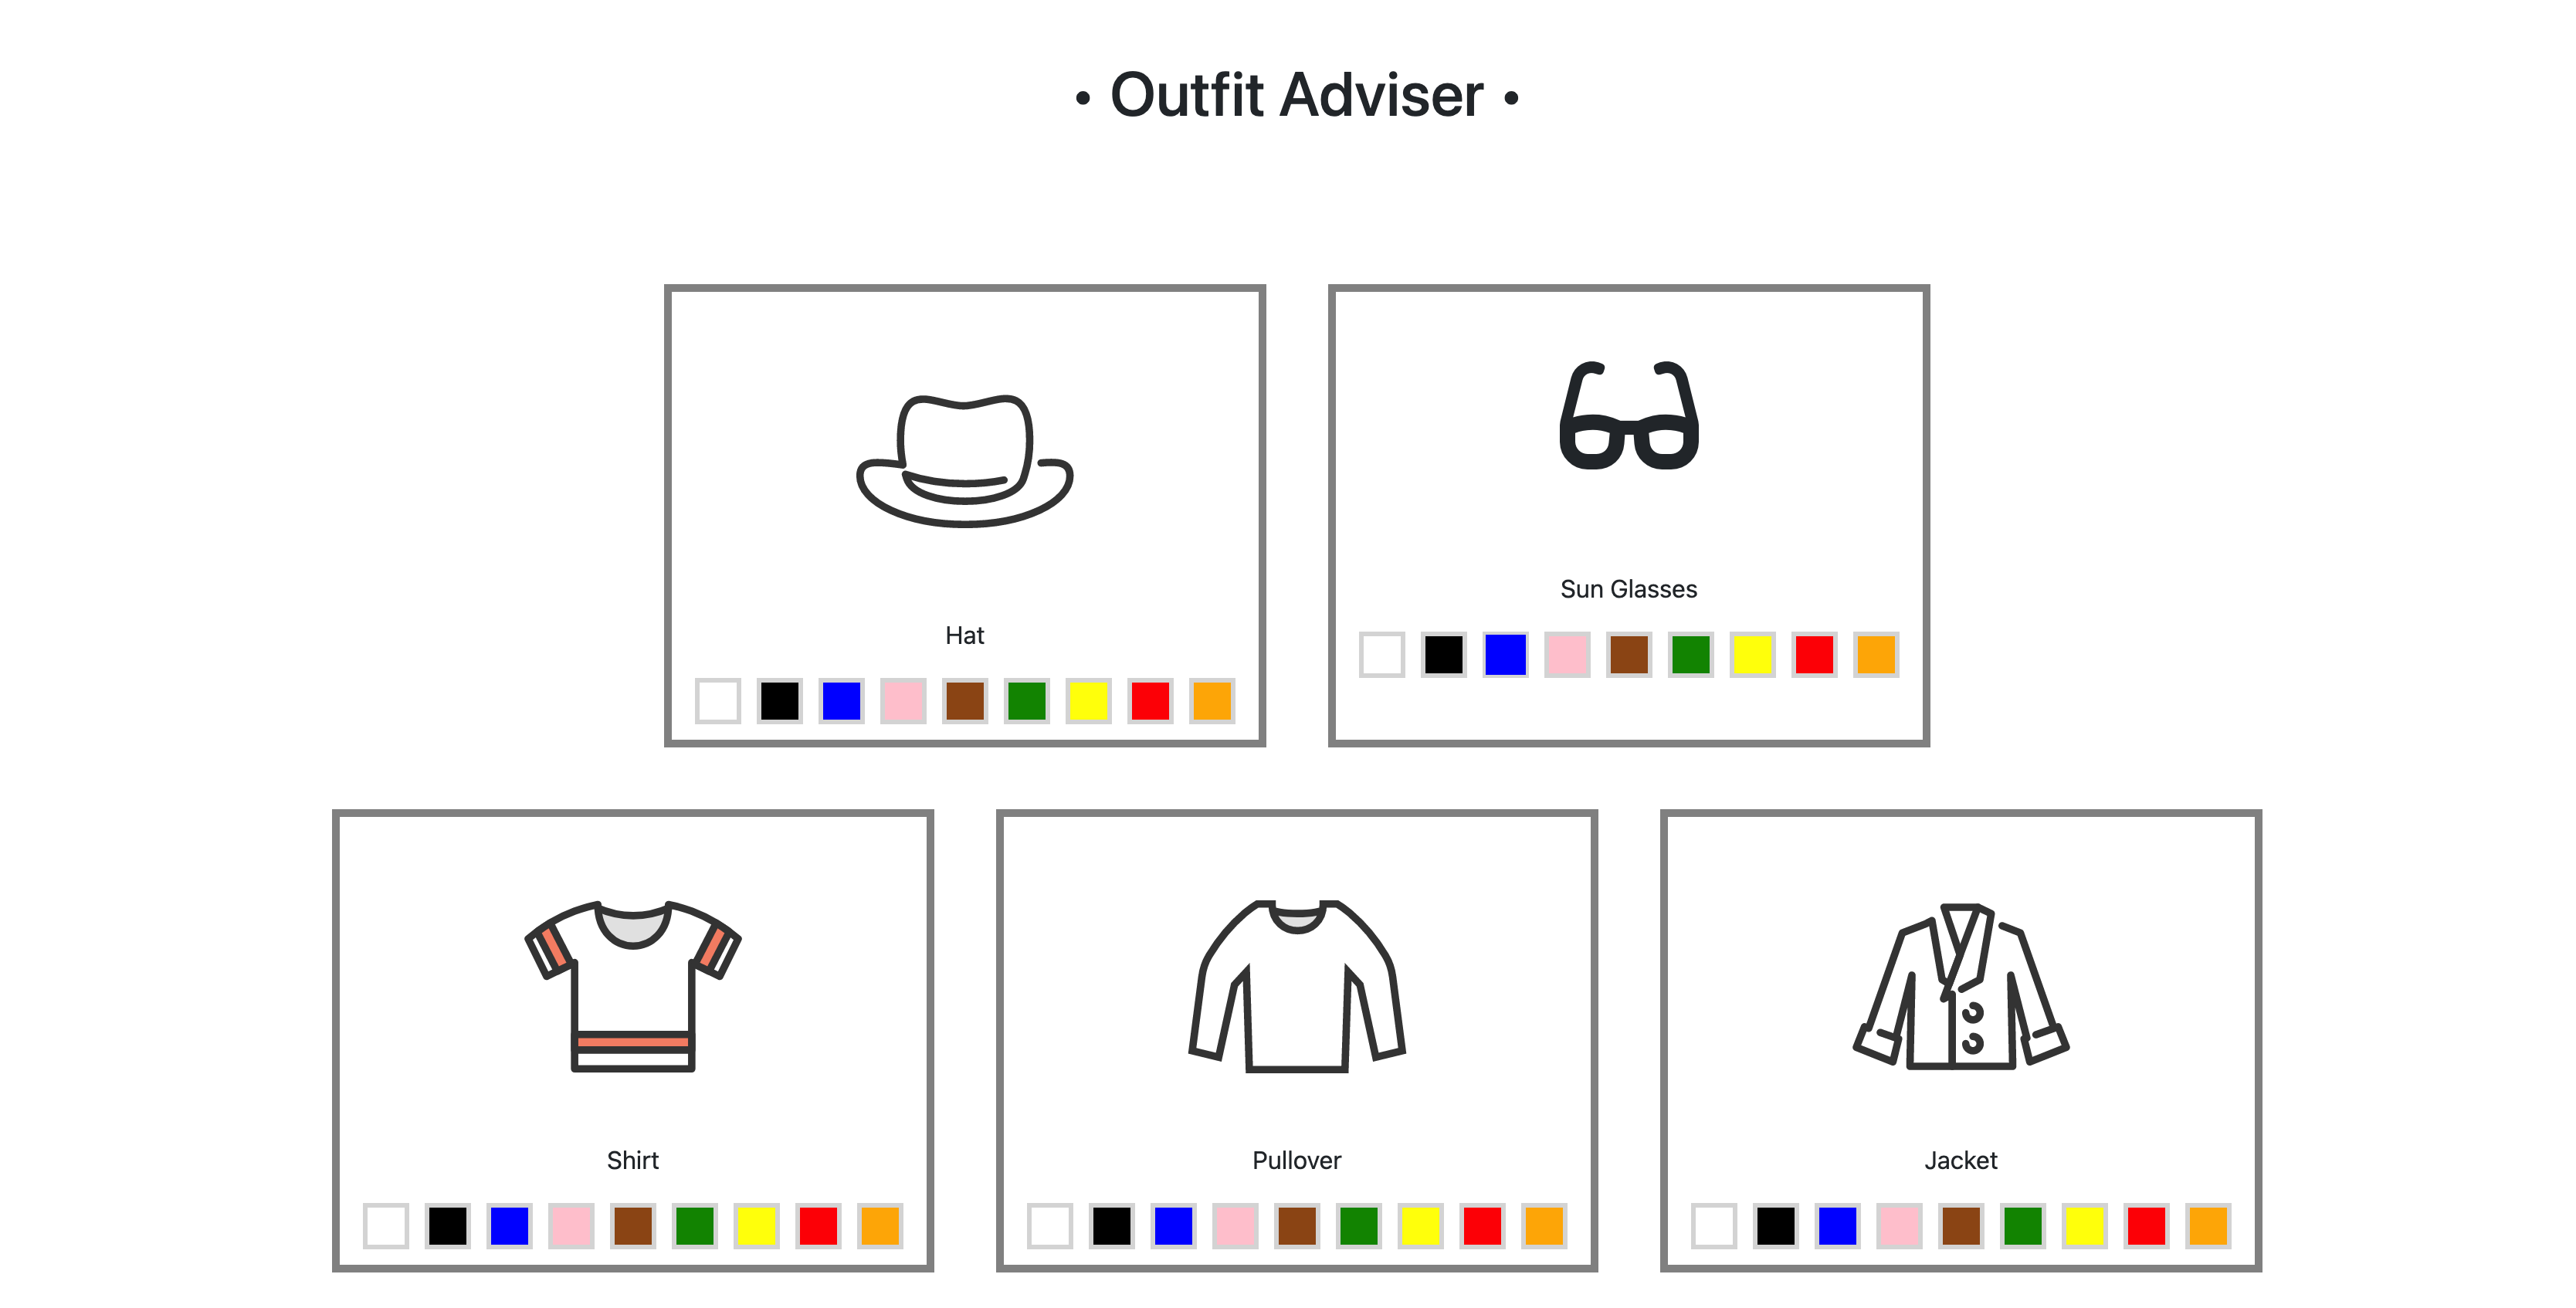
\includegraphics[width=\linewidth]{1-interface.png}
  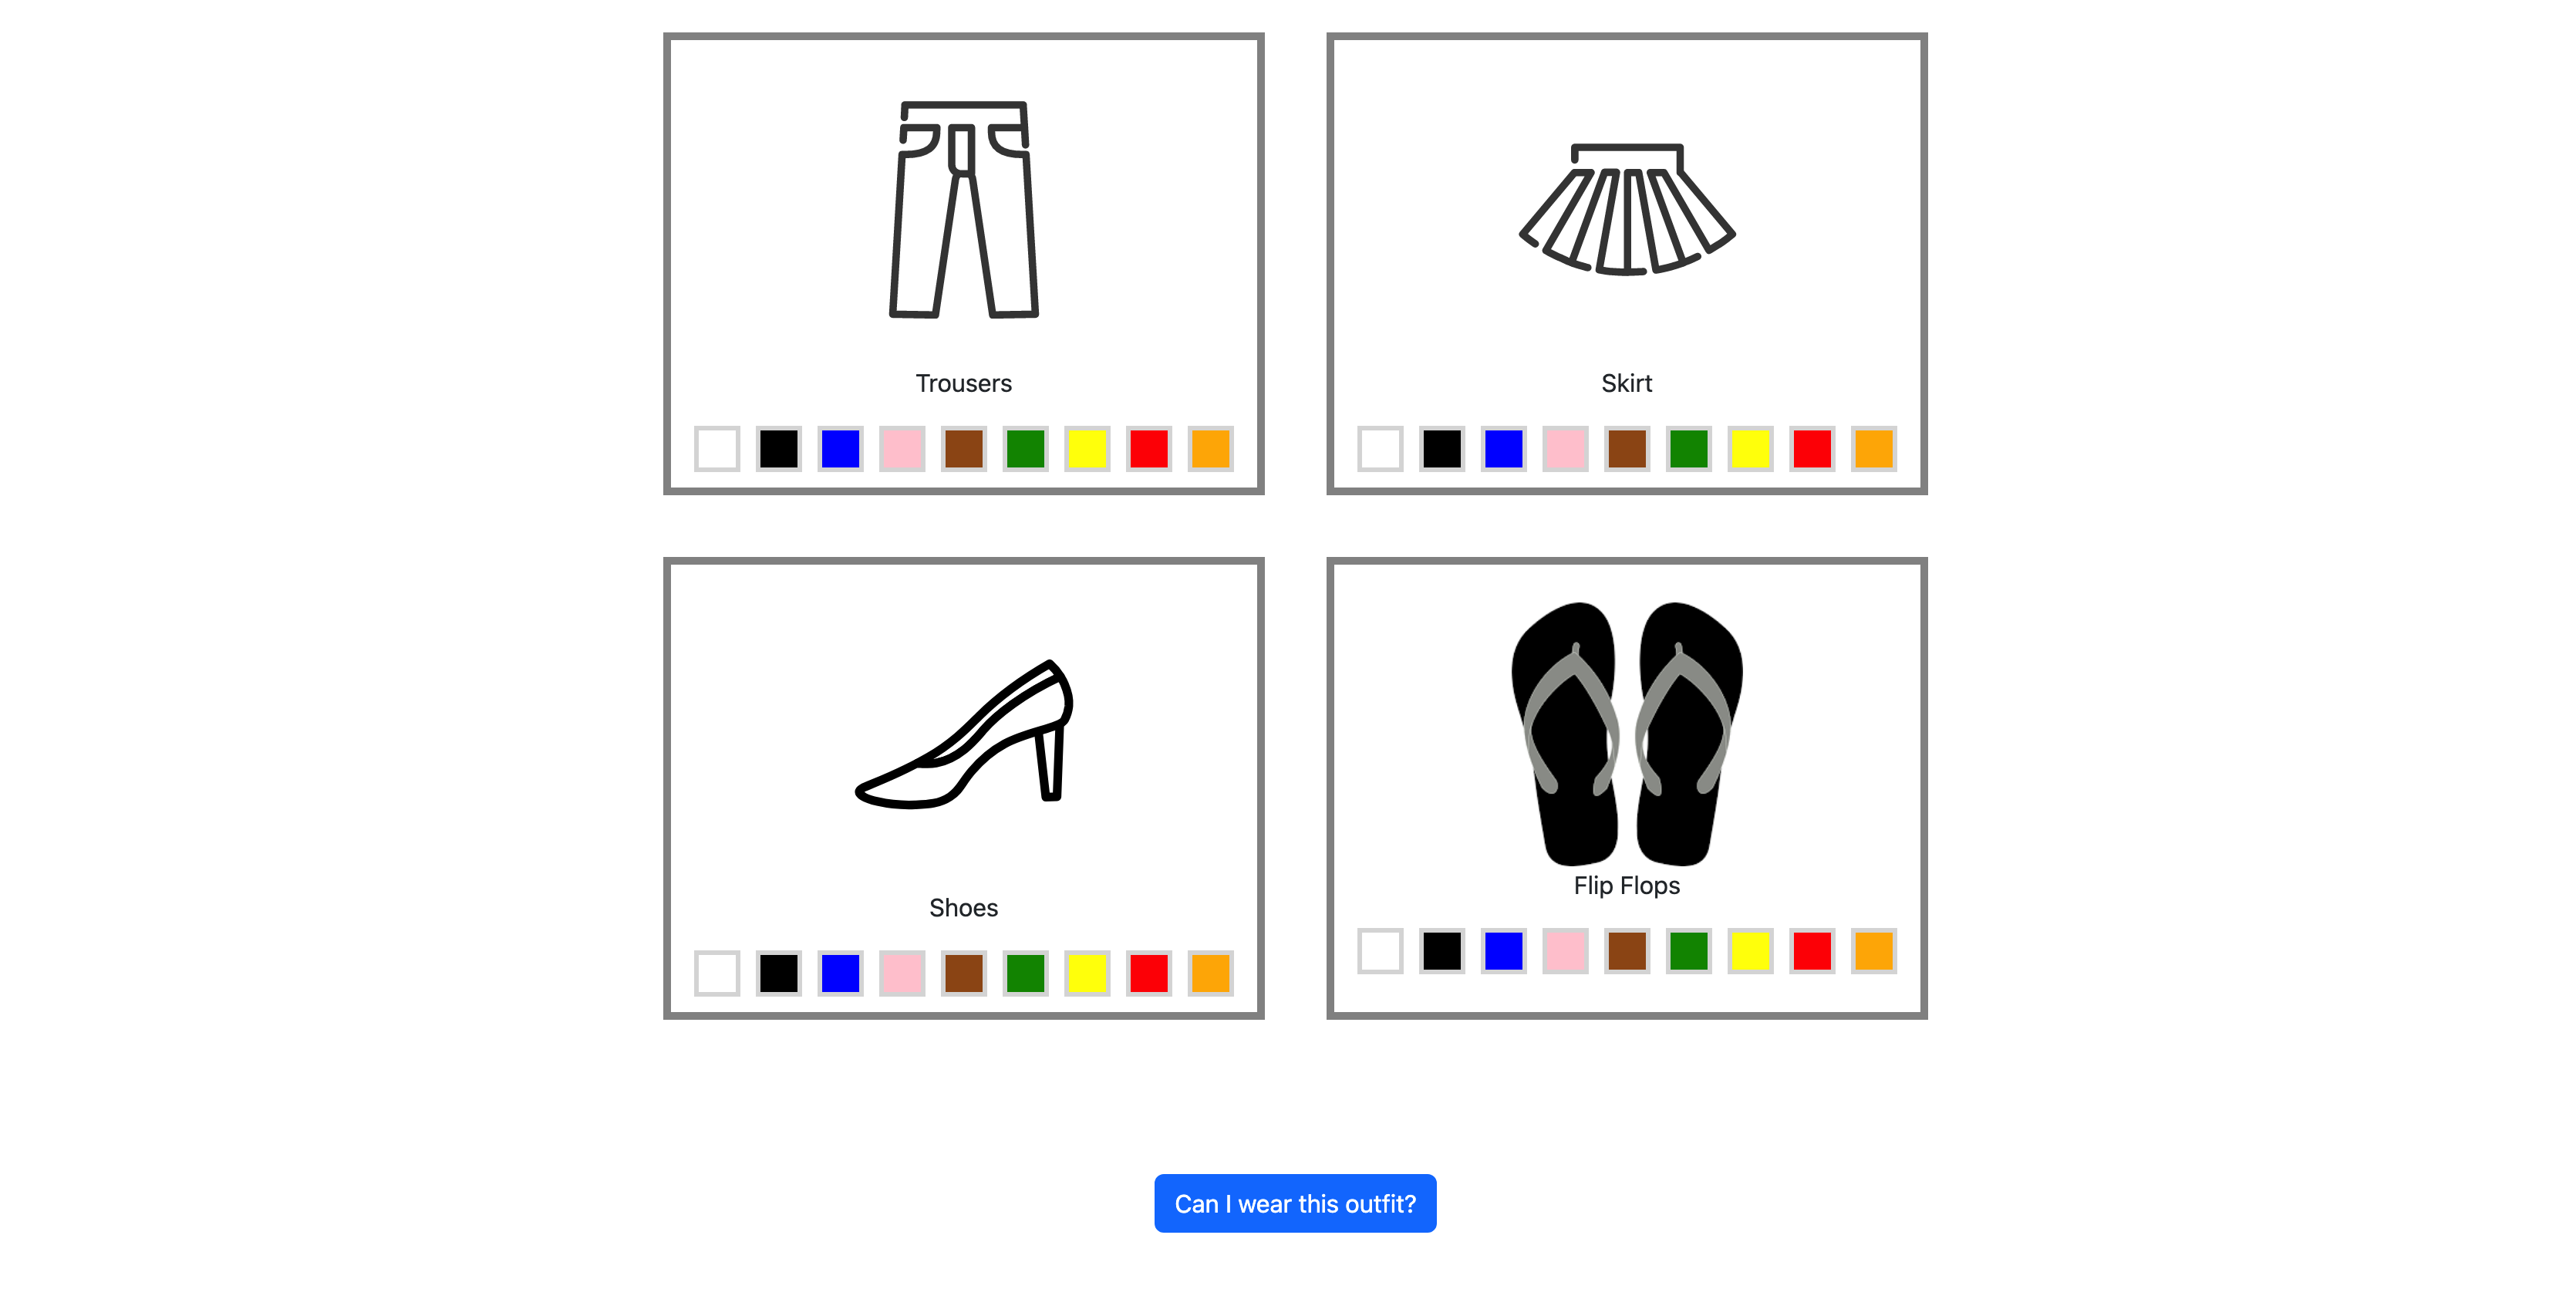
\includegraphics[width=\linewidth]{2-interface.png}
  \caption{Interface where you can decide how to wear}
  \label{interface}
\end{figure}

Once you select the outfit, you can click on "Can I wear this outfit?" and a message appears saying if your outfit satisfies the constraints as in picture \ref{is-ok}, or not as in picture \ref{not-ok}.

\begin{figure}
  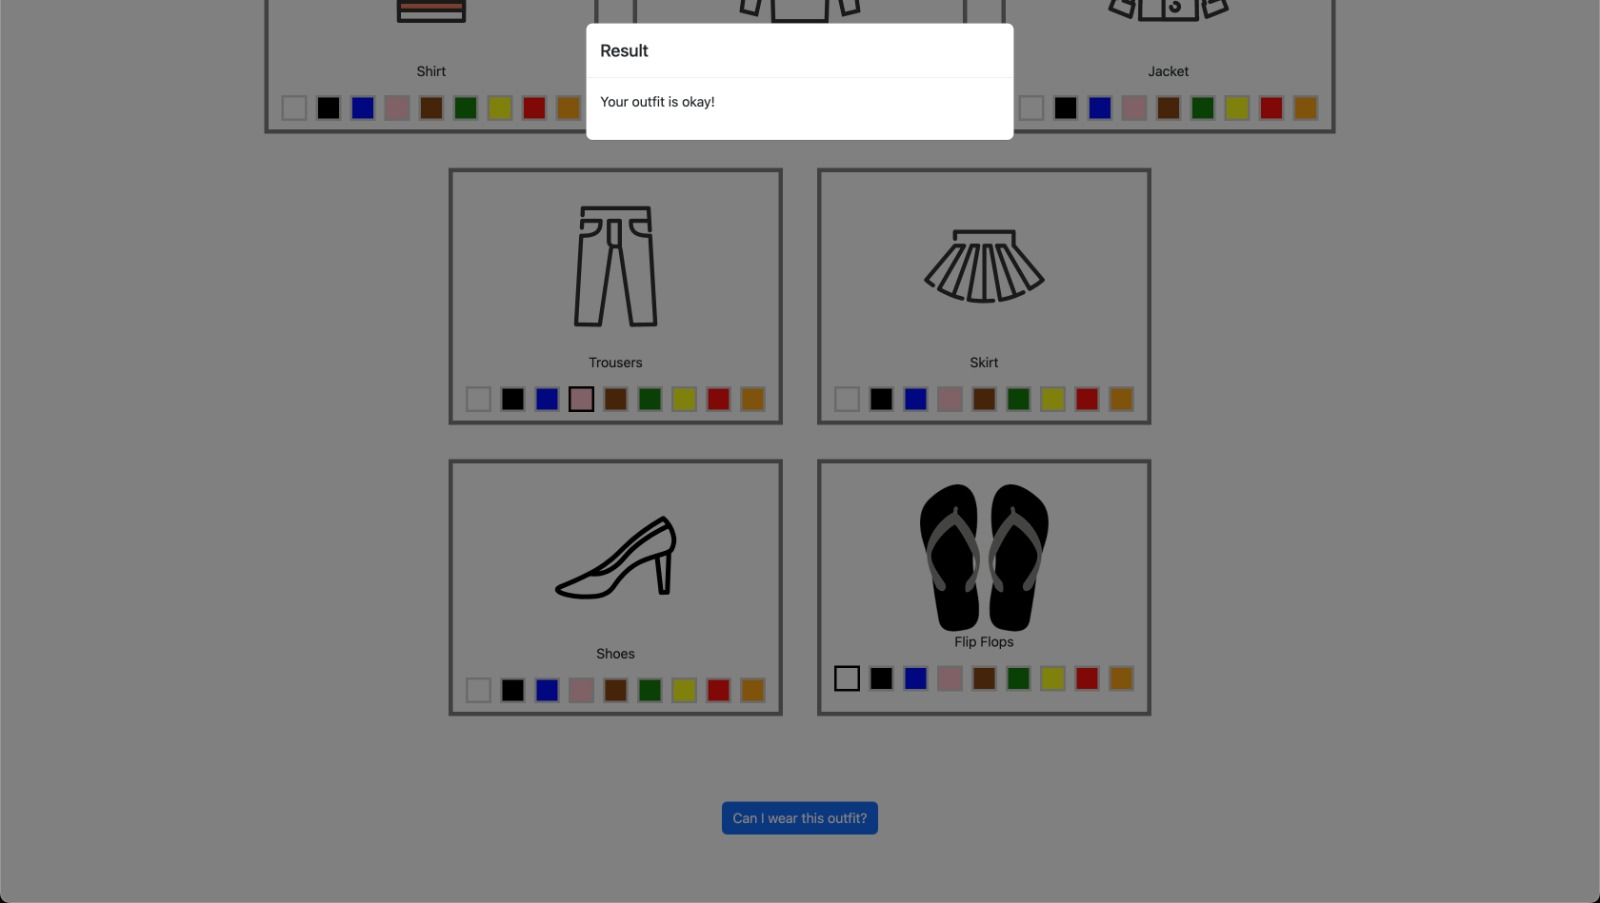
\includegraphics[width=\linewidth]{is-ok.jpg}
  \caption{Message saying your outfit satisfies the constrains.}
  \label{is-ok}
\end{figure}

\begin{figure}
  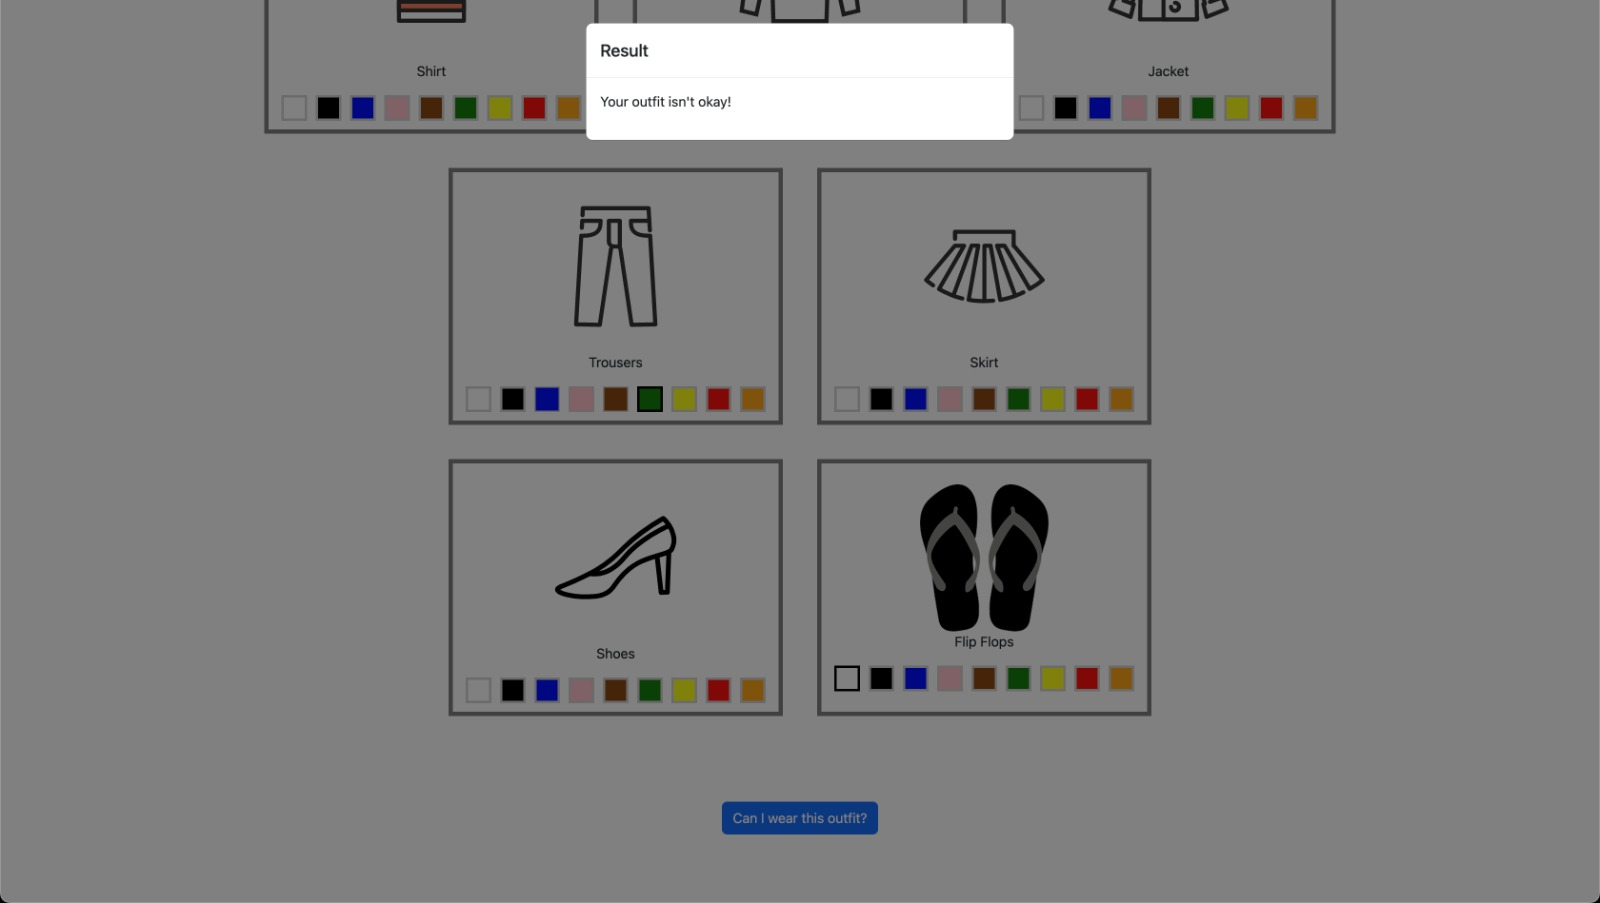
\includegraphics[width=\linewidth]{not-ok.jpg}
  \caption{Message saying your outfit doesn't satisfies the constrains.}
  \label{not-ok}
\end{figure}

\section{Design and Implementation}
We decided to implement the constraints as couples of clothes and colors since it's a simple and optimal solution. We chose these sets:


\begin{center}
	clothes = \{shirt, pullover, jacket, trousers, skirt, shoes, flipFlops, hat, sunglasses\}\\
	colors = \{white, black, blue, pink, brown, green, yellow, red, orange\}
\end{center}


\section{SAT solver}

As first step, we created two dictionaries for all the clothes and all the colors relatively. We defined a Solver and we added all the constraints into the Solver. Next step, we pass the input file - with the clothes and colors that the user wants to wear - to the Solver, in order to store them with an AND gate. In this way the Solver already know if the constraints (cloth and color) are satisfied or not. Last step is to check if the solver is SAT which succeeds, or not SAT which fails.  

The table of constrains we added, represented as boolean expression is the following:


\begin{center}
\begin{tabular}{|c|}
\hline
Boolean expression for constraints \\[0.1cm]
\hline 
$\neg$(skirt $\wedge$ trousers) \\[0.2cm]
$\neg$(shoes $\wedge$ flipFlops) \\[0.2cm]
$\neg$(pullover $\wedge$ jacket) \\[0.2cm]
$\neg$(pullover $\wedge$ flipFlops) \\[0.2cm]

(pullover $\rightarrow$ shirt) \\[0.2cm]
(jacket $\rightarrow$ shirt) \\[0.2cm]
(jacket $\rightarrow$ (shirt $\lor$ trousers)) \\[0.2cm]
((flipFlops $\lor$ sunglasses)  $\rightarrow$ hat)\\[0.2cm]
$\neg$(red $\wedge$ orange) \\[0.2cm]
$\neg$(pink $\wedge$ red) \\[0.2cm]
$\neg$(blue $\wedge$ green) \\[0.2cm]
$\neg$(brown $\wedge$ pink) \\[0.2cm]
$\neg$(pink $\wedge$ green) \\[0.2cm]
$\neg$(green $\wedge$ yellow) \\[0.2cm]
$\neg$(blue $\wedge$ yellow) \\[0.2cm]
$\neg$(red $\wedge$ green) \\[0.2cm]
$\neg$(brown $\wedge$ black) \\[0.2cm]

\hline
\end{tabular}
\end{center}

We wrote the entire code for the Solver in Python, precisely in file Solver.py. To implement it we used z3-solver library, and pandas to read the input file. 
\newpage
\section{Problems encountered}
At the beginning we had some problems implementing the solver because it was a new concept that we didn't know. After some searches on Google, we found out the library z3-solver and we smoothly implemented it. 

To process the input data with the constraints we used an AND gate instead of an OR, in order to satisfy every constrain.

\end{document}
